\chapter{Analysis of the $\lambda$~Orionis Region}


% some references to get things started:
%http://www.sea-astronomia.es/drupal/sites/default/files/archivos/tesis/Bayo_tesis.pdf
%that one from wikipedia using WISE data


	Having looked at AME vs. dust emission on a course scale, we now introduce our analysis of a particular region. The $\lambda$~Orionis molecular ring \footnote{Also known as the Meissa Ring}, shown in Figure \ref{fig:orionis-akari9} as it appears in 1$^{\circ}$ smoothed AKARI 9~$\mu$m data, indicates excess microwave emission attributed to AME \citep{planck15XXV}. At approx. 10$^{\circ}$ wide, we can see the outline of the structure even in the low (1$^{\circ}$ FWHM) resolution Planck-COMMANDER AME map. At this resolution,This is one of the only coherent structures on the sky with a well-resolved shape; the molecular cloud ring, perhaps originating from a supernova remnant is distinguishable from the ionized region at its center. . In order to shift towards an investigation of individual AME-prominent regions, we have carried out an initial comparison of the AME of this region with its mid to far-IR dust emission.

	Figure \ref{fig:orionis-img} shows the region in 12 photometric bands, from the mid to far IR. Contours indicate the region's shape in the Planck PR2 AME map. Figure \ref{fig:orionis-corr} shows IR to AME cross correlation plots, for all pixels within the 10$^{\circ}$ by 10$^{\circ}$ $\lambda$~Orionis region. The correlation is most clear for the shortest and for the longest wavelength bands, and weakens the most at around 60~$\mu$m. The weakening of the correlation score appears to come from brighter 25 to 90~$\mu$m emission within the ring, while the ring structure itself appears relatively consistent accross all bands.

\begin{figure*}
  \label{fig:orionis-akari9}
  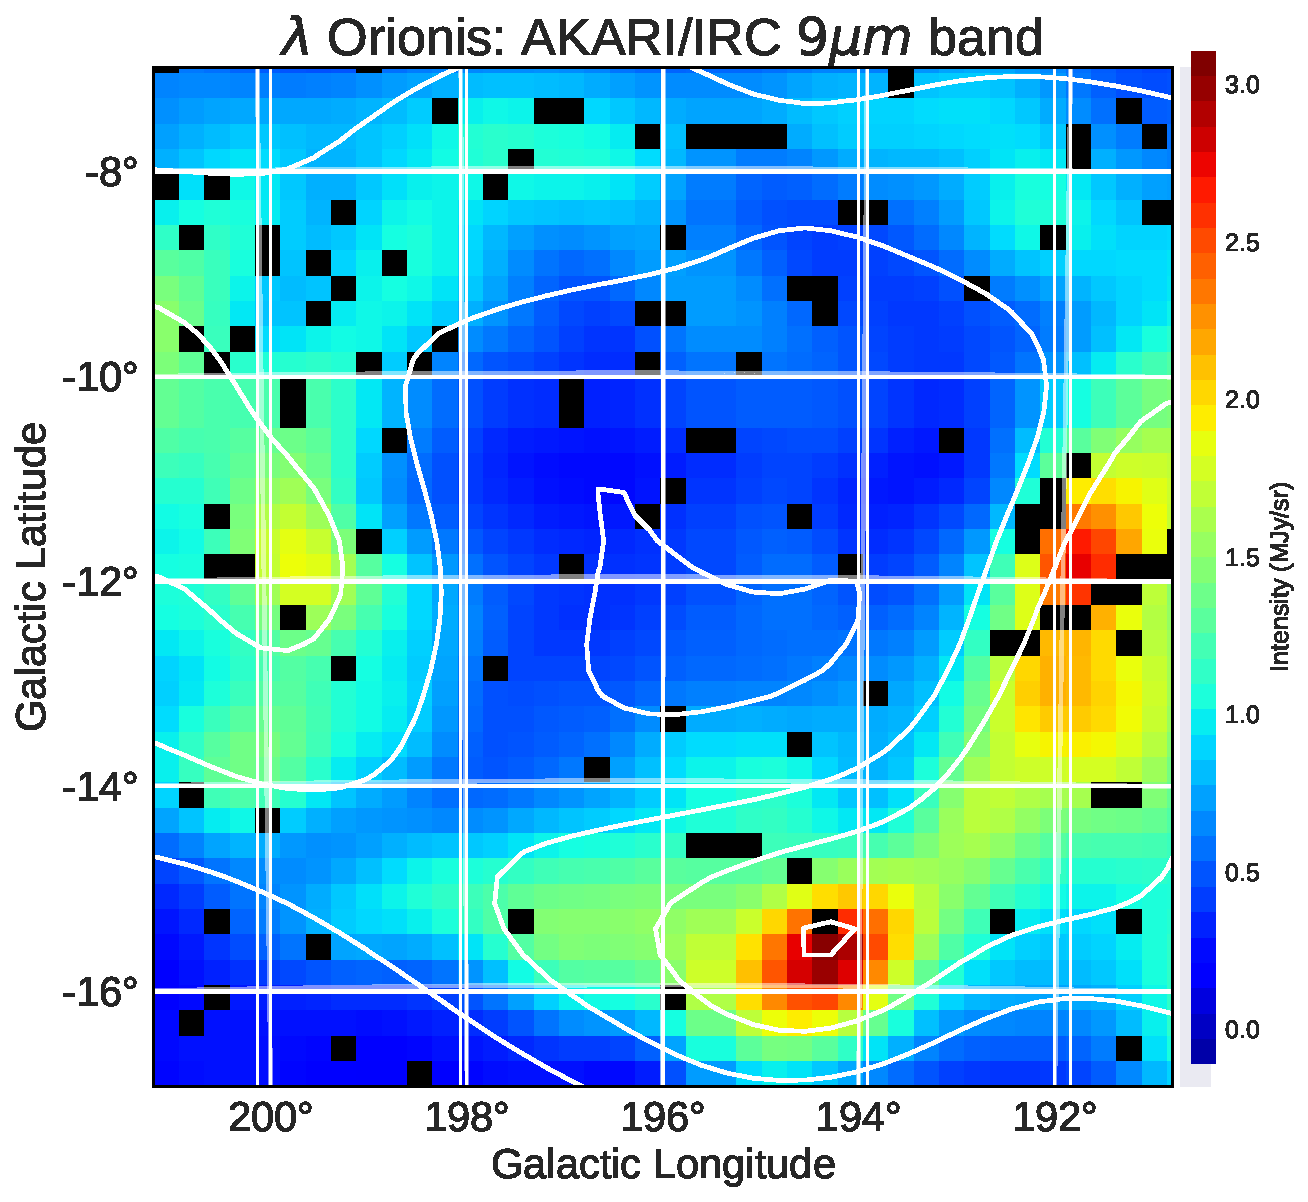
\includegraphics[width=150mm]{../Plots/LOri_akari9_AMEcont_1dres.pdf}
  \centering
  \caption{$\lambda$~Orionis as it appears in the AKARI 9~$\mu$m data. Contours indicate the AME, as given by the Planck PR2 AME map. The image is smoothed to a 1$^{\circ}$ PSF (much larger than the original 10 arcsec map. The $\lambda$~Orionis star itself is approximately located at the center of the image.
  %The dust wave structure, described by *citation needed*, is apparent, and seems to coincide with a local maxima in the PR2 AME contours. The units are MJy/sr. )
  }
\end{figure*}

\begin{figure*}
  \label{fig:orionis-img}
  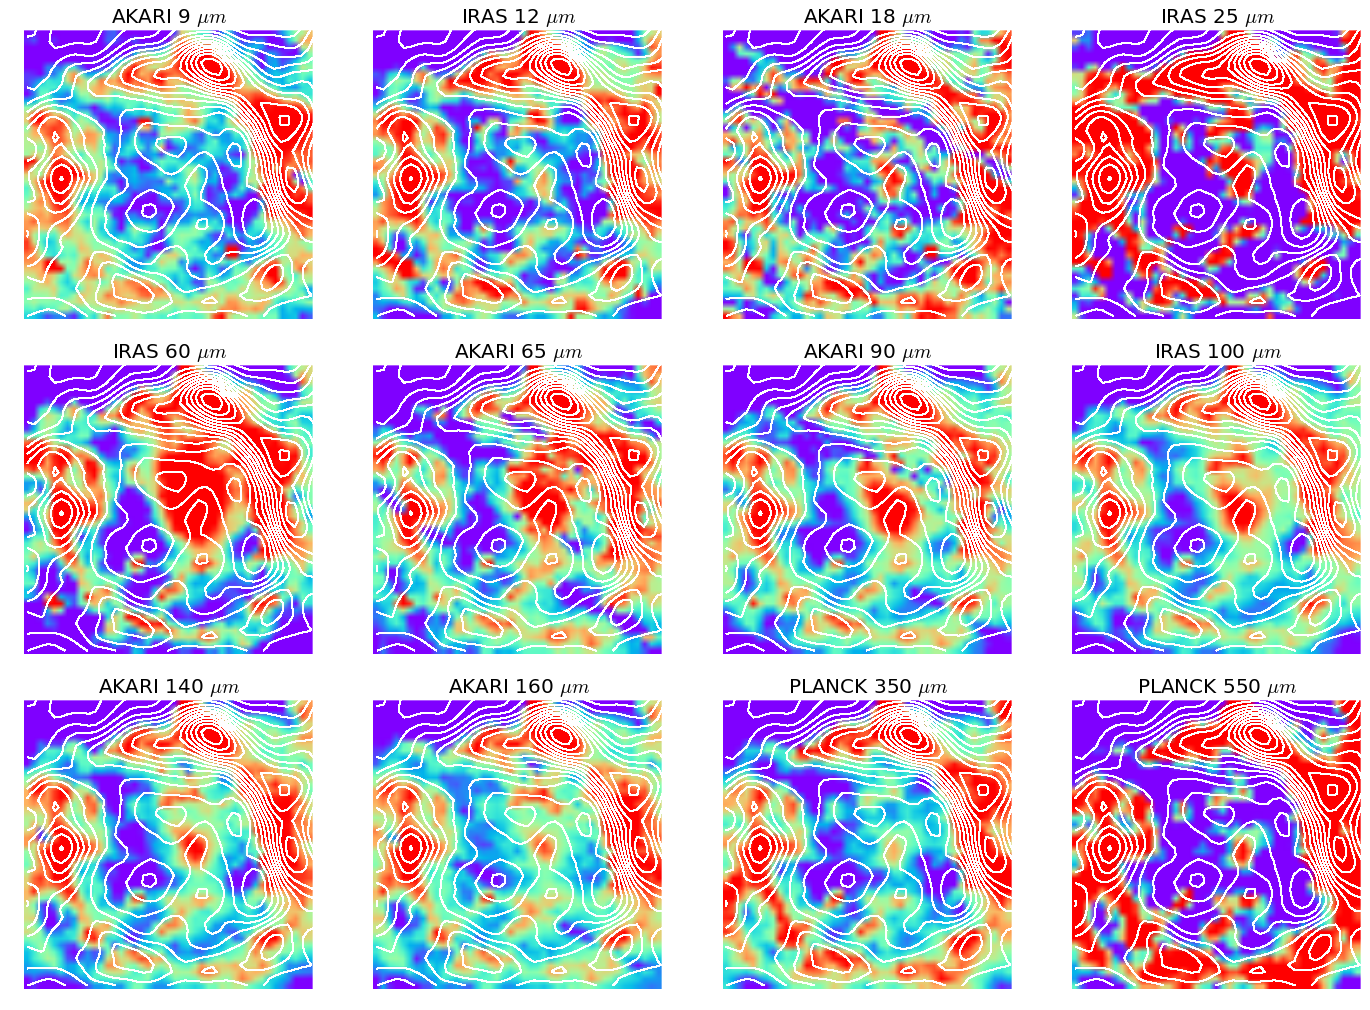
\includegraphics[width=170mm]{../Plots/lOrionis_grid_img.png}
  \centering
  \caption{A grid of thumbnails showing the $\lambda$~Orionis region's structure, at 12 wavelengths, along with AME contours (shown in white countours. Spatial correlation seems to be the best at the shortest and longest wavelengths (AKARI/IRC 9~$\mu$m and Planck/HFI 550~$\mu$m). The images are smoothed and interpolated for demonstration. Figure \ref{fig:orionis-akari9} demonstrates the actual pixel grid used for the SED fitting and intensity correlation tests.}
\end{figure*}

\begin{figure*}
  \label{fig:orionis-corr}
  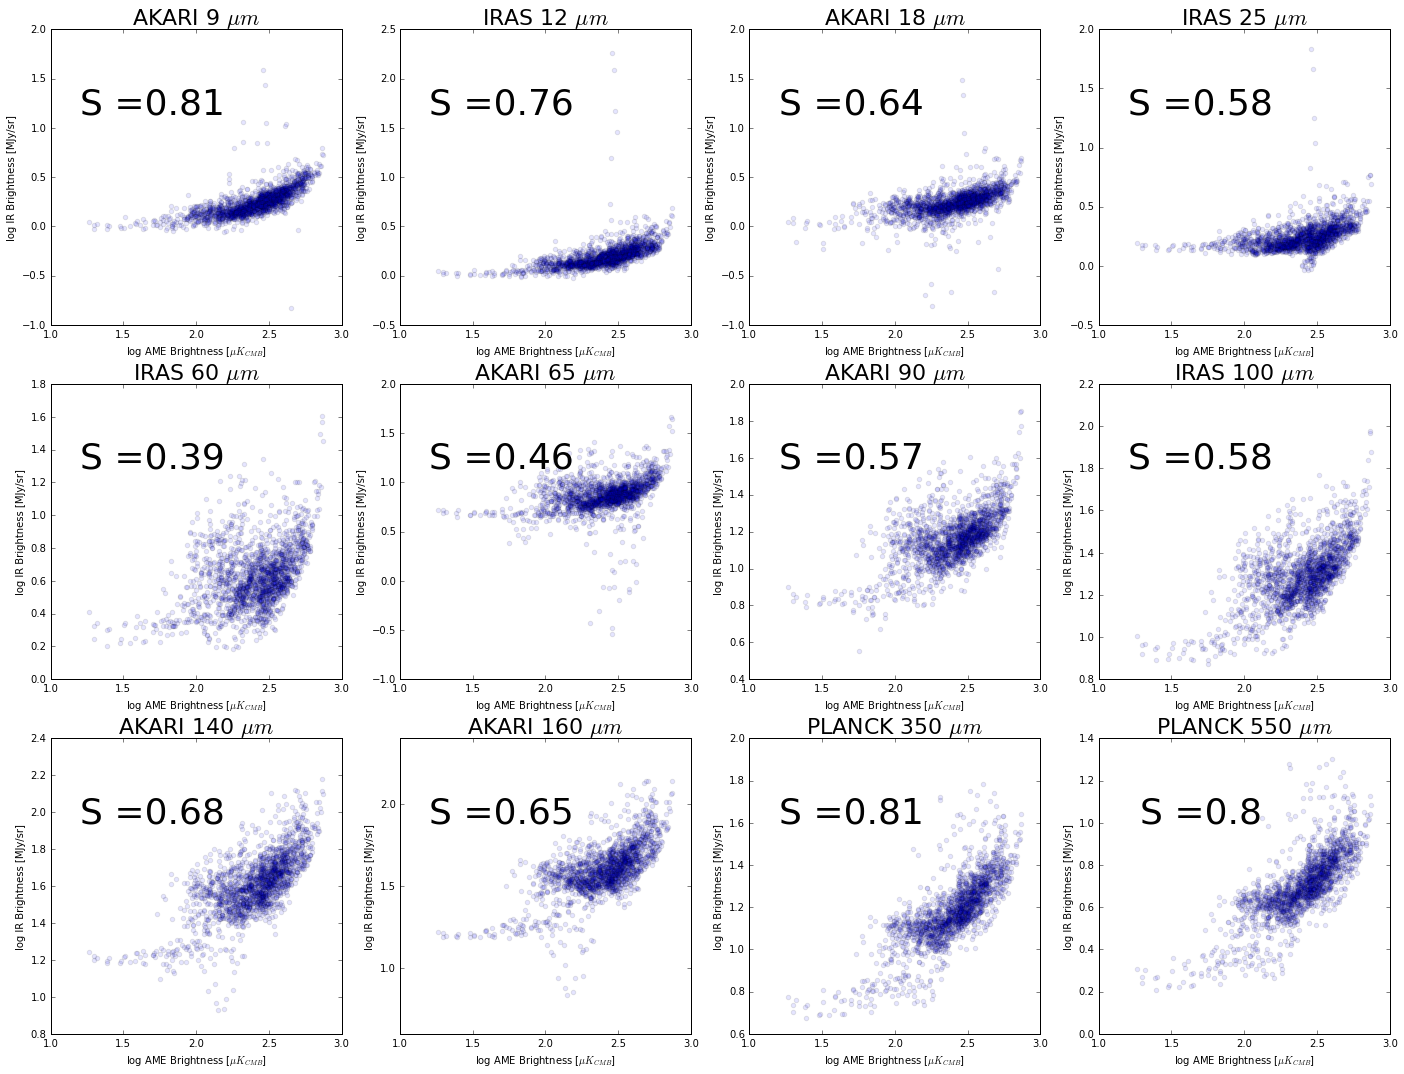
\includegraphics[width=170mm]{../Plots/orionis_correlations_AME.png}
  \centering
  \caption{Pixel cross-correlation for all pixels in the $\lambda$~Orionis cut-out region.  $S$ indicates the Spearman rank correlation coefficient for each plot.}
\end{figure*}

\subsubsection{SED Fitting}

We performed a full dust SED fitting on the LOri photometry, according to the \cite{galliano11} dust model. We used a mixture of amorphous carbon and silicate dust. Indeed, this dust mixture is more emissive than the standard silicate-graphite \citep{draine07}, by a factor of 2-3. As was shown by Herschel, in the LMC \citep{galliano11}, and by Planck, in the Milky Way \citep{planck16}, this increase of emissivity is necessary to have a proper fit of the sub-mm emission. We assume that the radiation field heating this dust mixture is the Galactic ISRF \citep{math83}, scaled by a factor $U$. We also assume, following \cite{dale01}, that the dust is exposed to a distribution of starlight intensity, distributed as:

\begin{equation}
   \label{eq:U}
     dM_{dust}\propto{} U^{-\alpha}dU
\end{equation}

between $U_{min}$ and $U_{max}$, where $U_{min}$, $U_{max}$ and $\alpha{}$ are free parameters. An old stellar population template (PEGASE; \citep{fioc97}) is added to this SED in order to model the near-IR emission. We perform a simple least-squares analysis. For the vast majority of the samples, the fits are reasonable, with the $\chi{}^{2}$ distribution shown in Fig. \ref{fig:AME_PCXVvsPR2}.
